\section{Interessengruppen}

\begin{center}
  \begin{figure}[ht]
    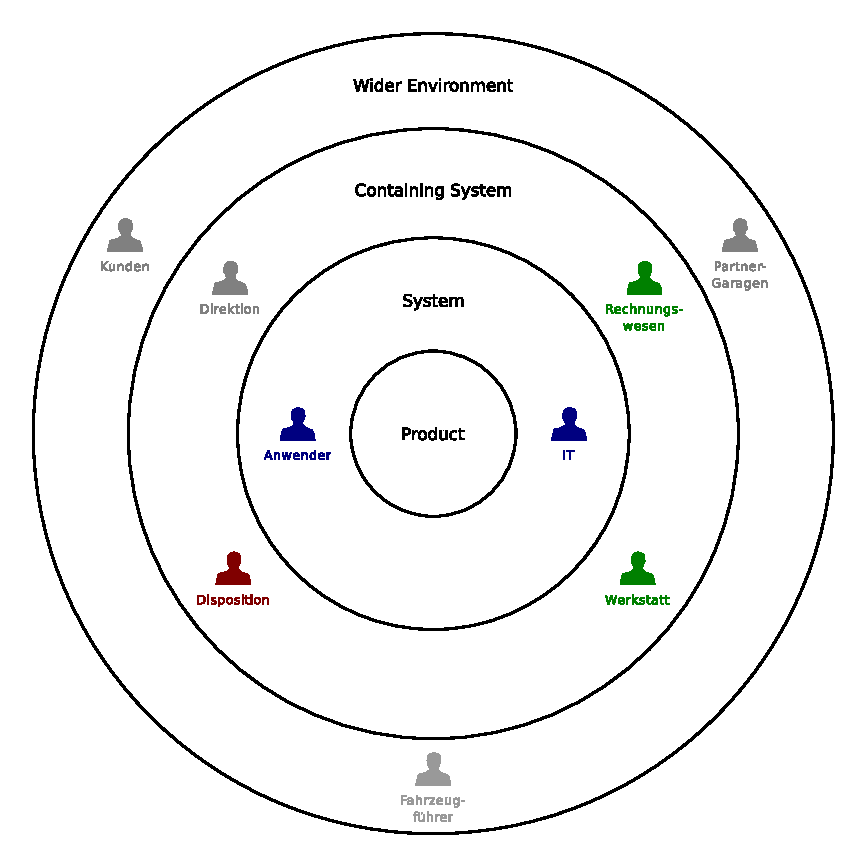
\includegraphics{graphics/onion.pdf}
    \caption{Onion-Diagramm der Nutz AG Steakholders}
    \label{fig:awesome_image}
  \end{figure}
\end{center}

\newpage
\subsection{Anwender}
Die Anwender sind für die Verwaltung des Fahrzeugparks zuständig. Es handelt sich meist um Angestellte mit einem kaufmännischen Hintergrund. Sie möchten mit dem System bestehende Abläufe möglichst einfach ausführen. 


\subsection{IT}
Die IT besteht aus 3 Mitarbeitern im Support. Komplexere Aufgaben werden mit externen Partnern realisiert. Ein AS400-System ist im Einsatz und der Wartungsvertrag läuft in 14 Monaten aus. Dies ist der Endtermin aus Sicht der IT. Der IT-Verantwortliche hat klare Vorstellungen an das neue System, welche teilweise ausserhalb des Einsatzgebietes liegen. Die Software soll umfangreich und trotzdem einfach nutzbar sein. Die Wartungsarbeiten an Serversystemen soll für den Support minimiert werden.

\subsection{Rechnungwesen}
Das Rechnungswesen möchte die Kosten um 20\% mit dem Projekt senken. Das Berichtswesen soll ausgebaut werden. Die Zahlungsmoral soll verbessert werden, beispielsweise durch eine "realtime" Debitorenbuchhaltung. Ebenfalls soll eine Auswertung der Debitoren nach Kunden, Kundengruppen, Fahrzeugkategorien möglich sein. Diese Auswertung dient den Führungskräften zur Kommunikation gegen Innen und Aussen. Ziel für das Rechnungswesen ist es den Gewinn zu optimieren.

\subsection{Disposition}
Die Disposition ist verantwortlich, dass sich die Fahrzeuge zum richtigen Zeitpunkt am richtigen Ort befinden. Die interne Organisation ist den Beteiligten klar. Bestehende Arbeitsabläufe sollen möglichst nicht verändert werden, da diese bereits mehrmals optimiert wurden.

\subsection{Direktion}
Der Direktor hat noch kein konkretes Budget erstellt. Die Obergrenze für das Projekt befindet sich zwischen 600'000 - 800'000 CHF. Er möchte keine Unruhe mit dem Projekt stiften, da er bald in Pension geht.

\subsection{Weitere Stakeholder}
Die Fahrzeuge dürfen nur im Inland eingesetzt werden. Wir vermuten wegen Versicherungsbedingungen und fehlendem Pannendienst. \\
Die Garagen müssen im Vorfeld über den Einsatz des Mietfahrzeugs in Ihrer Region informiert werden. Diese möchten für entsprechende Pannen im Vorfeld disponieren. \\
Die Kunden erwarten einen reibungslosen Ablauf bei der Miete der Fahrzeuge. Umständliche Formalitäten und lange Wartezeiten sollten möglichst vermieden werden.